% ### Uses XeLaTeX ### %
% ### Needs beamer-master ### %
\documentclass[aspectratio=169]{beamer} %. Aspect Ratio 16:9
\usetheme{AI2} % beamerthemeSprace.sty
% DATA FOR FOOTER
\date{2020}
\title{Deep Learning HPC}
\author{}
\institute{Advanced Institute for Artificial Intelligence (AI2)}
\begin{document}
% ####################################
% FIRST SLIDE 						:: \SliTit{This is the Title of the Talk}{A. B. Name}{Sprace}
% SUB-TITLE SLIDE 					:: \SliSubTit{<title>}{<explanation}
% SUB-SUB-TITLE SLIDE				:: \SliSubSubTit{<title>}{<explanation}
% SLIDE WITH TITLE 					:: \SliT{Title}{Content}
% SLIDE NO TITLE 						:: \Sli{Content} 
% SLIDE DOUBLE COLUMN WITH TITLE 	:: \SliDT{Title}{First Column}{Second Column}
% SLIDE DOUBLE COLUMN NO TITLE 		:: \SliD{First Column}{Second Column}
% SLIDE ADVANCED WITH TITLE 			:: \SliAdvT{Title}{Content}
% SLIDE ADVANCED NO TITLE 			:: \SliAdv{Content}
% SLIDE ADVANCED DOUBLE WITH TITLE 	:: \SliAdvDT{Title}{First Column}{Second Column}
% SLIDE ADVANCED DOUBLE NO TITLE 	:: \SliAdvD{First Column}{Second Column}
% SLIDE BLACK						:: \Black{ <Content> }
% SLIDE WHITE						:: \White{ <Content> }
% ITEMIZATION 						:: \begin{itemize}  \iOn{First} \iTw {Second} \iTh{Third} \end{itemize}
% COMMENT TEXT				 		:: \note{<comment>}
% SECTION 							:: \secx{Section} | \secxx{Sub-Section}
% BOLD SPRACE COLOR				:: \bfs{<text>}
% TABLE OF CONTENT					:: \tocitem{<title>}{<content>}
% LEFT ALIGN EQUATION				:: \begin{flalign*}  & <equation> &   \end{flalign*}
% CENTER ALIGN EQUATION	S			:: \begin{gather*} <equations>  \end{gather*}
% SLASH								:: \slashed{<>}
% BAR								:: \barr{<letter>} instead of \bar{<letter>}
% THEREFORE						:: use \portanto (larger and bold}
% 2 or 3 MATH SYMBOLS				:: \overset{<up>}{<down>} &  \underset{<below>}{\overset{<above>}{<middle>}}  
% INSERT TEXT IN FORMULA			:: \ins{<text>}
% EXERCISE							:: \exe{<exercise #>}{<exercise text>}
% SUGGESTED READING BOX			:: \sug{<references>}
% CITATION							:: \cittex{<citation>}
% CITATION DOUBLE COLUMN 			:: \cittexD{<citation>}
% TEXT POSITION						:: \texpos{<Xcm>}{<Ycm>}{<text>} origin = center of slide : x right | y down
% REFERENCE AT BOTTOM  S/D SLIDE		:: \refbotS{<reference>} \refbotD{<reference>}
% HIDDEN SLIDE						:: \hid
% COLOR BOX 						:: \blu{blue} + \red{rec} + \yel{yellow} + \gre{green} + \bege{beige}
% FRAME 							:: \fra{sprace} \frab{blue} \frar{red} + \fray{yellow} + \frag{green}		
% FIGURE 							:: \img{X}{Y}{<scale>}{Figure.png} 
% FIGURE							:: \includegraphics[scale=<scale>]{Figures/.png}
% FIGURE DOUBLE SLIDE NO TITLE		::  \img{-4}{0.5}{<scale>}{Figure.png} % Image 1st half
%									::  \img{4}{0.5}{<scale>}{Figure.png} % Image 2nd half
% FIGURE DOUBLE SLIDE WITH TITLE		::  \img{-4}{0}{<scale>}{Figure.png} % Image 1st half
%									::  \img{4}{0}{<scale>}{Figure.png} % Image 2nd half
% INCLUDING SWF (Flash)				:: \usepackage{media9} and \includemedia >> USE ACROBAT <<
%%%%%%%%%%%%%%%%%%%%%%%%%%%%%%%%%%%%%%%%%%%%%%%%%%
% ###############################################################################
% FIRST SLIDE
\SliTit{Deep Learning}{Advanced Institute for Artificial Intelligence -- AI2}{https://advancedinstitute.ai}


% SLIDE ADVANCED  WITH TITLE
\SliAdvT{Introdução a Deep Learning}{ 

Agenda

\begin{itemize}
  \iOn{Inteligência Artificial}
  \iOn{Introdução a Deep Learning}
  \iOn{Keras}
  \iOn{Representação de dados}
  \iOn{Exemplos de Aplicações em Redes Neurais}
\end{itemize}

}

\SliAdvT{O que é IA}{

\begin{itemize}
\iOn{Inteligência Artificial é uma grande área da ciência}

\iOn{Diversas vertentes da IA buscam avançar a ciência com reapeito a automatizar tarefas intelectuais normalmente realizadas por seres humanos}

\iOn{Atualmente, um campo estratégico para desenvolvimento de tecnologia }

\end{itemize}

}

\SliAdvT{O que é IA}{
O que é Inteligência?

\begin{itemize}
\iOn{Habilidade de aprender, contemplar, pensar e raciocinar}
\iOn{Mentalidade, senso}
\iOn{Discernimento, julgamento, sabedoria}
\end{itemize}
}


\SliAdvT{O que é IA}{
O que é Inteligência?


Nossas mentes contêm processos que nos capacitam a
solucionar problemas que consideramos difíceis.

Inteligência é o nome que damos a qualquer um destes processos que ainda não compreendemos

—Marvin Minsky
}

\SliAdvT{O que é IA}{
As abordagens para o estudo de IA se dividem em 4 categorias:

\begin{itemize}
  \iOn{Sistemas que pensam como seres humanos}
  \iTw{Modelagem cognitiva}
  \iTw{Programa de computador capaz de implementar o raciocínio humano}
  \iOn{Sistemas que pensam racionalmente}
   \iTw{Utilização de lógica formal para modelar a forma de resolver problemas}
  \iOn{Sistemas que agem como seres humanos}
  \iTw{Teste de Turing}
  \iOn{Sistemas que agem racionalmente}
\end{itemize}
}

\SliAdvT{O que é IA}{
Comportamento racional

\begin{itemize}
\iOn{Agir corretamente = fazer o que é esperado para atingir seus objetivos, dada a informação disponível}
\iOn{Não necessariamente involve pensamentos (raciocínios lógicos)}
\iOn{O raciocínio lógico deve ser usado para alcançar um objetivo.}
\end{itemize}
}

\SliAdvT{Deep Learning}{ 

\begin{itemize}
\iOn{Buscar representações úteis para os dados de entrada
Em um espaço pré-definido de possibilidades  (Pode ser um espaço grande)}
\iOn{Usando como critério o sucesso de realizar a representação}

\iOn{Tais passos permitem resolver diversas tarefas intelectuais, desde o reconhecimento de fala até a condução autônoma}
\end{itemize}

}

\SliAdvT{Deep Learning}{ 
O Deep learning é um subcampo específico do aprendizado de máquina

\begin{itemize}
\iOn{Abordagem de representação de aprendizado a partir de dados que enfatiza o aprendizado de camadas sucessivas de representações}

\iOn{outras abordagens ao aprendizado de máquina tendem a se concentrar no aprendizado de apenas uma ou duas camadas de representações dos dados (shallow learning)}

\iOn{No aprendizado profundo, essas representações em camadas são (quase sempre) aprendidas através de modelos chamados redes neurais, estruturadas em camadas literais empilhadas}


\end{itemize}
}
\SliAdvT{Deep Learning}{ 

\begin{center}
    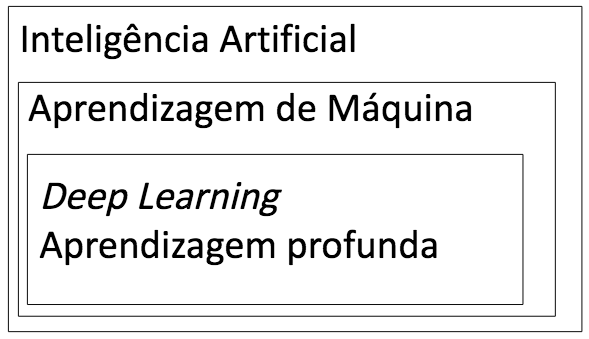
\includegraphics[scale=0.60]{figuras/DL.png}     
\end{center}
}

\SliAdvT{Deep Learning}{ 
\begin{itemize}
\iOn{A construção do modelo se baseia na observação da entrada e mapeamento da entrada para uma saída.}
\iOn{Tal mapeamento é feito associando um valor a cada peso associado a cada camada}
\iOn{Encontrar os pesos corretos de cada camada é desafiador}
\end{itemize}

}

% SLIDE ADVANCED  WITH TITLE
\SliAdvT{Representação de Dados}{ 

Uma etapa essencial e complexa de utilizar modelos de deep learning é a representação de dados

\begin{itemize}
  \iOn{Imagem}
  \iOn{Texto}
  \iOn{Audio}
  \iOn{Vídeo}
  \iOn{Sequências}
  \iTw{Fenômenos caracterizados ao longo de um período de tempor}
  \iTh{variação de clima ao longo do tempo}
  \iTh{uma sequência de palavras indicando uma classe}
  \iTh{uma sequência de frames indicando uma situação}
  \iTh{uma sequência de cores indicando uma variação no ambiente}
\end{itemize}


}


\SliAdvT{Deep Learning}{ 
\begin{itemize}
\iOn{Uma forma de controlar o processo de atribuir pesos as camadas é utilizar a função loss}
\iOn{Essa função retorna um score de distância entre o valor real e o valor predito}
\iOn{Com base no valor obtido pela função loss um otimizador faz os ajustes adequados nos pesos, usando um algoritmo chamado backpropagation}
\end{itemize}

}

\SliAdvT{Deep Learning}{ 

\begin{itemize}
\iOn{Inicialmente os neuronios da rede recebem valores aleatórios}
\iOn{o processo de ajustes de peso é feito por um algoritmo iterativo.}

\iOn{Em cada passo são executadas as seguintes funções}
\iTw{Entrada é submetida a rede neural e um valor predito é gerado para cada item da base de dados}
\iTw{Função loss calcula a distância entre valor predito e real de cada item da base de entrada}
\iTw{Função otimizadora utiliza valor retornado na função loss e atualiza o peso}
\iOn{A cada passo do algortimo o retorno da função loss é minimizado, e os pesos começam a representar de forma mais efetiva os dados de entrada}
\end{itemize}
A rotina iterativa de atualização dos pesos também é chamada de época
}

\SliDT{Deep Learning}
{
Passos de uma época
\begin{itemize}
\iOn{1) Dados submetidos as camadas (X)}
\iOn{2) Respostas geradas (y)}
\iOn{3) Função para comparar a perda entre predito e real}
\iOn{4) Diferença é enviada a função otimizadora}
\iOn{5) Otimizador atualiza os pesos de cada camada}
\end{itemize}

}{
\begin{center}
    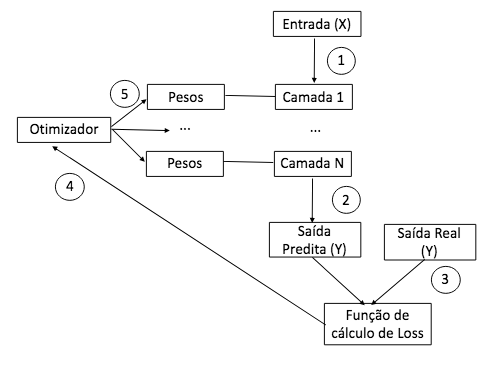
\includegraphics[scale=0.45]{figuras/epoca.png}     
\end{center}
}

\SliAdvT{Deep Learning}{ 

Diversos parâmetros podem ser definidos na rotina de aprendizagem

\begin{itemize}
\iOn{Número de camadas}
\iTw{Quantidade de neurônios por camada}
\iTw{Função de ativação de cada camada}
\iTw{Parâmetros de cada função de ativação}
\iOn{Tamanho do Batch}
\iOn{Critério de parada do laço de treinamento}
\iOn{Função Otimizadora}
\iOn{Função Loss}
\iOn{Métrica}
\end{itemize}
}

%\SliAdvT{Deep Learning}{ 
%Diversas APIs tem sido desenvolvidas
%}
%\iOn{A seleção da entrada pode ser feita da seguinte forma:}
%\iTw{Uma linha do dataset for vez}
%\iTw{Um subconjunto de linhas do dataset for vez}
%

%\begin{itemize}
%\iOn{A execução de cada época é iniciada a partir dos dados de entrada (X), que podem ser divididos da seguinte forma}
%\iTw{Execução de Uma época para cada linha da base de dados}
%\iTw{Execução de Uma época para subconjuntos de linhas da base de dados}

%\iOn{A diferença de usar um método ou outro tem impacto no desempenho e na acurácia do modelo}
%}


\SliAdvT{Keras}{ 

\begin{itemize}
  \iOn{API de redes neurais de alto nível}
  \iOn{Utiliza recursos do TensorFlow, CNTK ou Theano;}
  \iOn{Foco em experimentação rápida}
  \iOn{Compatível com: Python}
      
\end{itemize}

}

%\SliAdvT{Keras}{ 
%Iniciando modelo 
%\begin{itemize}
%  \iOn{sequential}
%\end{itemize}
%}
%\SliAdvT{Keras}{ 
%Criando camadas
%\begin{itemize}
%  \iOn{Dense}
%\end{itemize}
%}

%\SliAdvT{Keras}{ 
%Compilando e treinando o modelo
%\begin{itemize}
%  \iOn{fit}
%  \iOn{train}
%\end{itemize}
%}

%\SliAdvT{Keras}{ 
%Avaliando a qualidade
%\begin{itemize}
%  \iOn{evaluate}
%  \iOn{predict}
%\end{itemize}
%}


\end{document}
